\begin{frame}{Automatic Feature Selection}
It can be a good idea to reduce the number of features to only the most useful ones

\begin{itemize}
    \item Simpler models that generalize better (less overfitting)
    \begin{itemize}
        \item Curse of dimensionality (e.g. kNN)
        \item Even models such as RandomForest can benefit from this
        \item Sometimes it is one of the main methods to improve models (e.g. gene expression data)
    \end{itemize}
    
    \item Faster prediction and training
    \begin{itemize}
        \item Training time can be quadratic (or cubic) in number of features
    \end{itemize}
    
    \item Easier data collection, smaller models (less storage)
    
    \item More interpretable models: fewer features to look at
\end{itemize}
\end{frame}


\begin{frame}{Example: bike sharing}
\begin{itemize}
    \item The Bike Sharing Demand dataset shows the amount of bikes rented in Washington DC
    \item Some features are clearly more informative than others (e.g. temp, hour)
    \item Some are correlated (e.g. temp and feel\_temp)
    \item We add two random features at the end
\end{itemize}

\begin{figure}
    \centering
    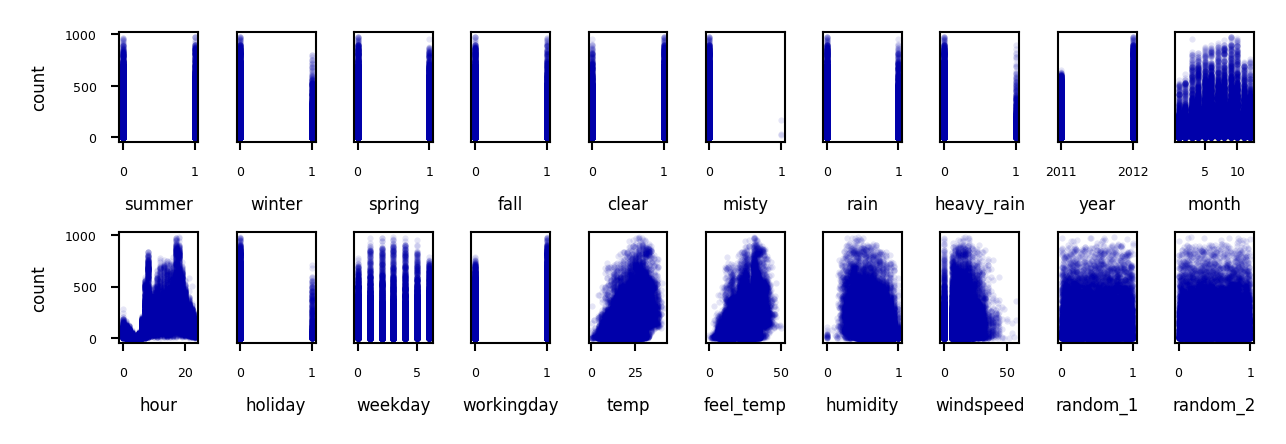
\includegraphics[width=0.95\textwidth,keepaspectratio]{images/pre-processing/bike_sharing.png}
\end{figure}
\end{frame}


\begin{frame}[allowframebreaks]{Unsupervised feature selection}
\begin{itemize}
    \item Variance-based
    \begin{itemize}
        \item Remove (near) constant features
        \begin{itemize}
            \item Choose a small variance threshold
        \end{itemize}
        \item Scale features before computing variance!
        \item Infrequent values may still be important
    \end{itemize}

    \item Covariance-based
    \begin{itemize}
        \item Remove correlated features
        \item The small differences may actually be important
        \begin{itemize}
            \item You don't know because you don't consider the target
        \end{itemize}
    \end{itemize}
\end{itemize}

\begin{figure}
    \centering
    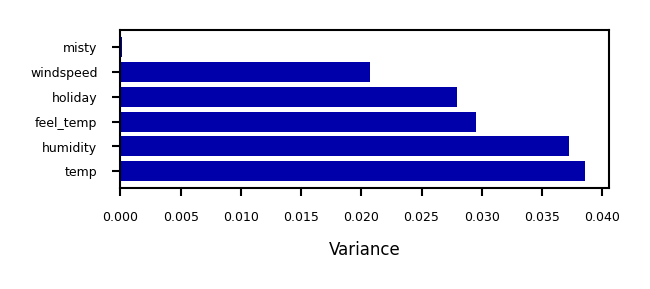
\includegraphics[width=0.75\textwidth,keepaspectratio]{images/pre-processing/variance-based.png}
\end{figure}
\end{frame}

\begin{frame}[allowframebreaks]{Covariance based feature selection}
\begin{itemize}
    \item Remove features $X_i$ (= $\mathbf{X}_{\cdot,i}$) that are highly correlated (have high correlation coefficient $\rho$)
\end{itemize}

\[
\rho(X_1, X_2) = \frac{\text{cov}(X_1, X_2)}{\sigma(X_1)\sigma(X_2)} = 
\frac{\frac{1}{N-1} \sum_i (X_{i,1} - \overline{X_1})(X_{i,2} - \overline{X_2})}
{\sigma(X_1)\sigma(X_2)}
\]

\begin{itemize}
    \item Should we remove \texttt{feel\_temp}? Or \texttt{temp}? Maybe one correlates more with the target?
\end{itemize}

\begin{figure}
    \centering
    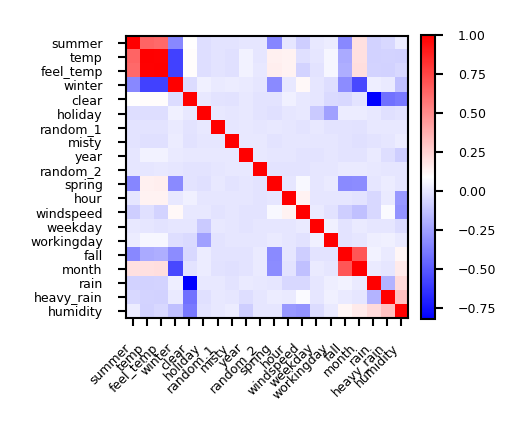
\includegraphics[width=0.85\textwidth,keepaspectratio]{images/pre-processing/covariance-based.png}
\end{figure}
\end{frame}

\begin{frame}{Supervised feature selection: overview}
\begin{itemize}
    \item Univariate: F-test and Mutual Information
    \item Model-based: Random Forests, Linear models, kNN
    \item Wrapping techniques (black-box search)
    \item Permutation importance
\end{itemize}
\end{frame}


\begin{frame}[allowframebreaks]{Univariate statistics (F-test)}
\begin{itemize}
    \item Consider each feature individually (univariate), independent of the model that you aim to apply
    \item Use a statistical test: is there a \textit{linear statistically significant relationship} with the target?
    \item Use F-statistic (or corresponding p value) to rank all features, then select features using a threshold
    \begin{itemize}
        \item Best $k$, best $k\%$, probability of removing useful features (FPR), \ldots
    \end{itemize}
    \item Cannot detect correlations (e.g. temp and feel\_temp) or interactions (e.g. binary features)
\end{itemize}

\begin{figure}
    \centering
    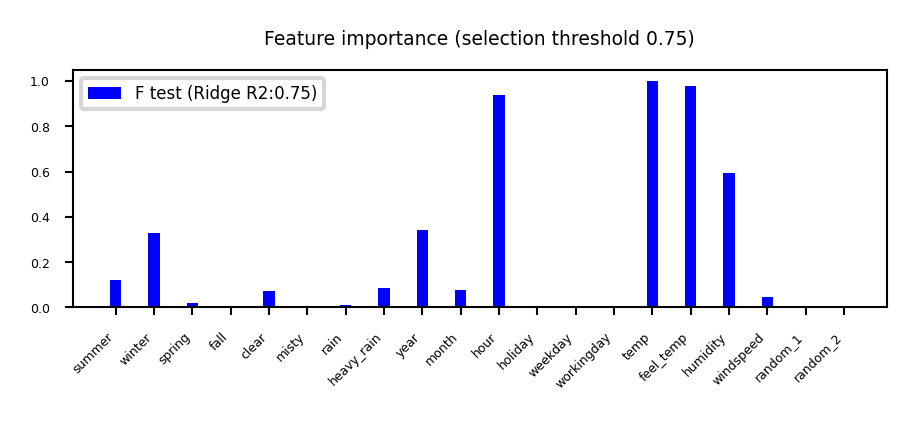
\includegraphics[width=0.85\textwidth,keepaspectratio]{images/pre-processing/F-test.png}
\end{figure}
\end{frame}

\begin{frame}[allowframebreaks]{F-statistic}
\begin{itemize}
    \item For regression: does feature $X_i$ correlate (positively or negatively) with the target $y$?
\end{itemize}

\[
\text{F-statistic} = \frac{\rho(X_i, y)^2}{1 - \rho(X_i, y)^2} \cdot (N - 1)
\]

\begin{itemize}
    \item For classification: uses ANOVA: does $X_i$ explain the between-class variance?
    \begin{itemize}
        \item Alternatively, use the $\chi^2$ test (only for categorical features)
    \end{itemize}
\end{itemize}

\[
\text{F-statistic} = \frac{\text{within-class variance}}{\text{between-class variance}} = \frac{\text{var}(\overline{X_i})}{\text{var}(X_i)}
\]

\begin{figure}
    \centering
    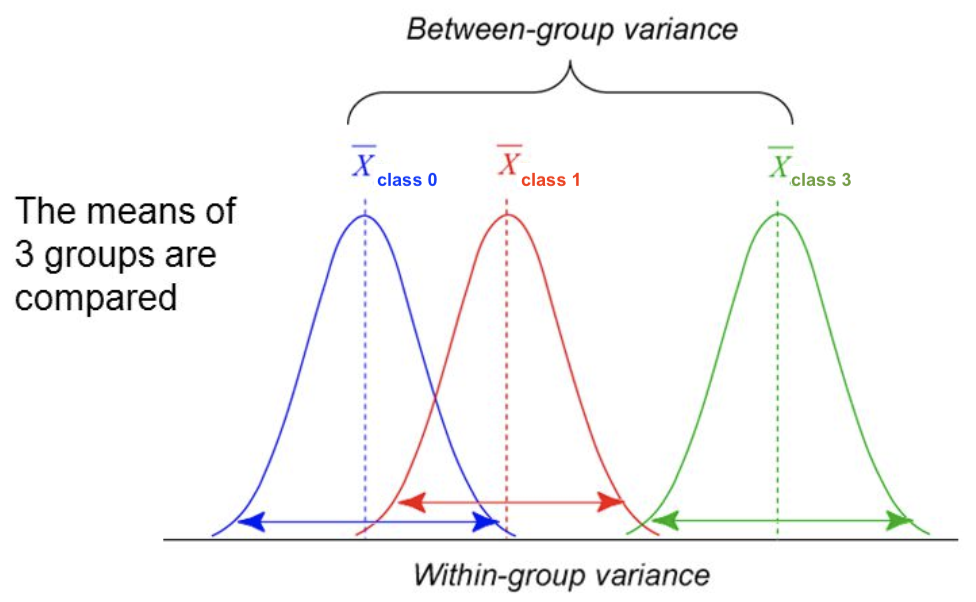
\includegraphics[width=0.85\textwidth,keepaspectratio]{images/pre-processing/fstatistic.png}
\end{figure}
\end{frame}

\begin{frame}[allowframebreaks]{Mutual information}
\begin{itemize}
    \item Measures how much information $X_i$ gives about the target $Y$. In terms of entropy $H$:
\end{itemize}

\[
MI(X, Y) = H(X) + H(Y) - H(X, Y)
\]

\begin{itemize}
    \item Idea: estimate $H(X)$ as the average distance between a data point and its $k$ Nearest Neighbors
    \begin{itemize}
        \item You need to choose $k$ and say which features are categorical
    \end{itemize}
    \item Captures complex dependencies (e.g. hour, month), but requires more samples to be accurate
\end{itemize}

\begin{figure}
    \centering
    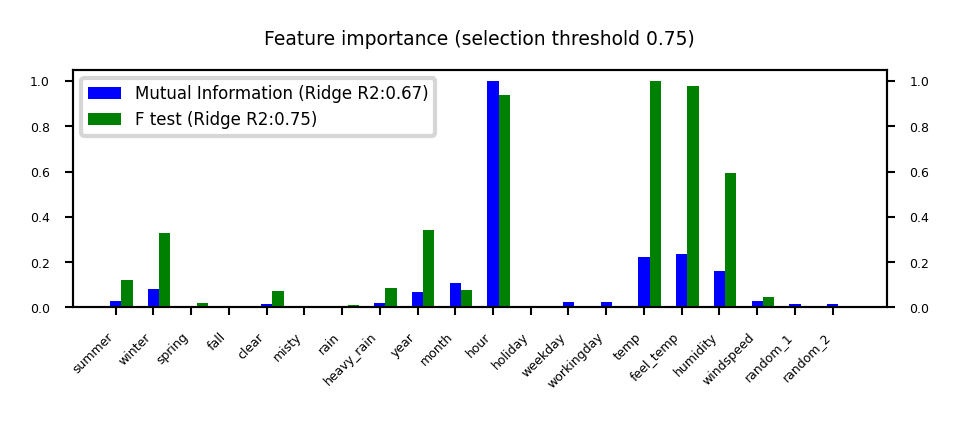
\includegraphics[width=0.9\textwidth,keepaspectratio]{images/pre-processing/mutual-information.png}
\end{figure}
\end{frame}



\begin{frame}[allowframebreaks]{Model-based Feature Selection}
\begin{itemize}
    \item Use a \textbf{tuned(!)} supervised model to judge the importance of each feature
    \begin{itemize}
        \item Linear models (Ridge, Lasso, LinearSVM, \ldots): features with highest weights (coefficients)
        \item Tree–based models: features used in first nodes (high information gain)
    \end{itemize}

    \item Selection model can be different from the one you use for final modelling

    \item Captures interactions: features are more/less informative in combination (e.g. winter, temp)

    \item RandomForests: learns complex interactions (e.g. hour), but biased to high cardinality features
\end{itemize}

\begin{figure}
    \centering
    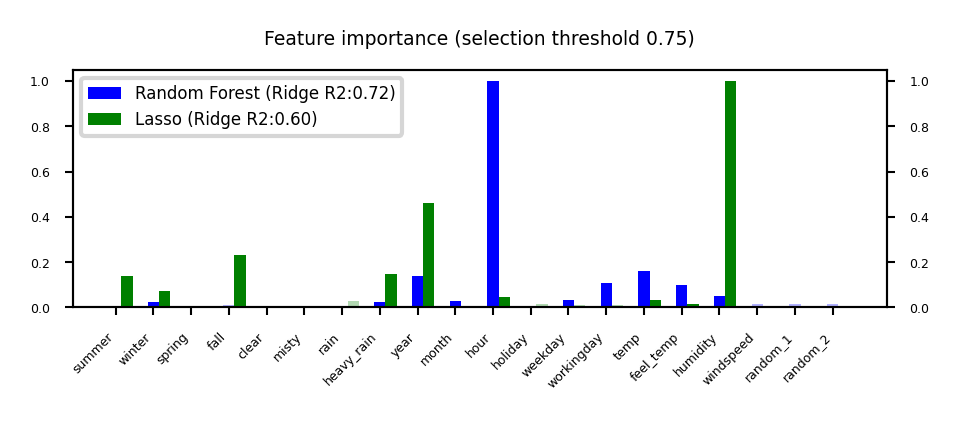
\includegraphics[width=0.9\textwidth,keepaspectratio]{images/pre-processing/model-based.png}
\end{figure}
\end{frame}


\begin{frame}[allowframebreaks]{Relief: Model-based selection with kNN}
\begin{itemize}
    \item For $l$ iterations, choose a random point $\mathbf{x}_i$ and find $k$ nearest neighbors $\mathbf{x}_k$
    \item Increase feature weights if $\mathbf{x}_i$ and $\mathbf{x}_k$ have different class (near miss), else decrease
\end{itemize}

\[
\mathbf{w}_i = \mathbf{w}_{i-1} + (\mathbf{x}_i - \text{nearMiss}_i)^2 - (\mathbf{x}_i - \text{nearHit}_i)^2
\]

\begin{itemize}
    \item Many variants: ReliefF (uses L1 norm, faster), RReliefF (for regression), \ldots
\end{itemize}

\begin{figure}
    \centering
    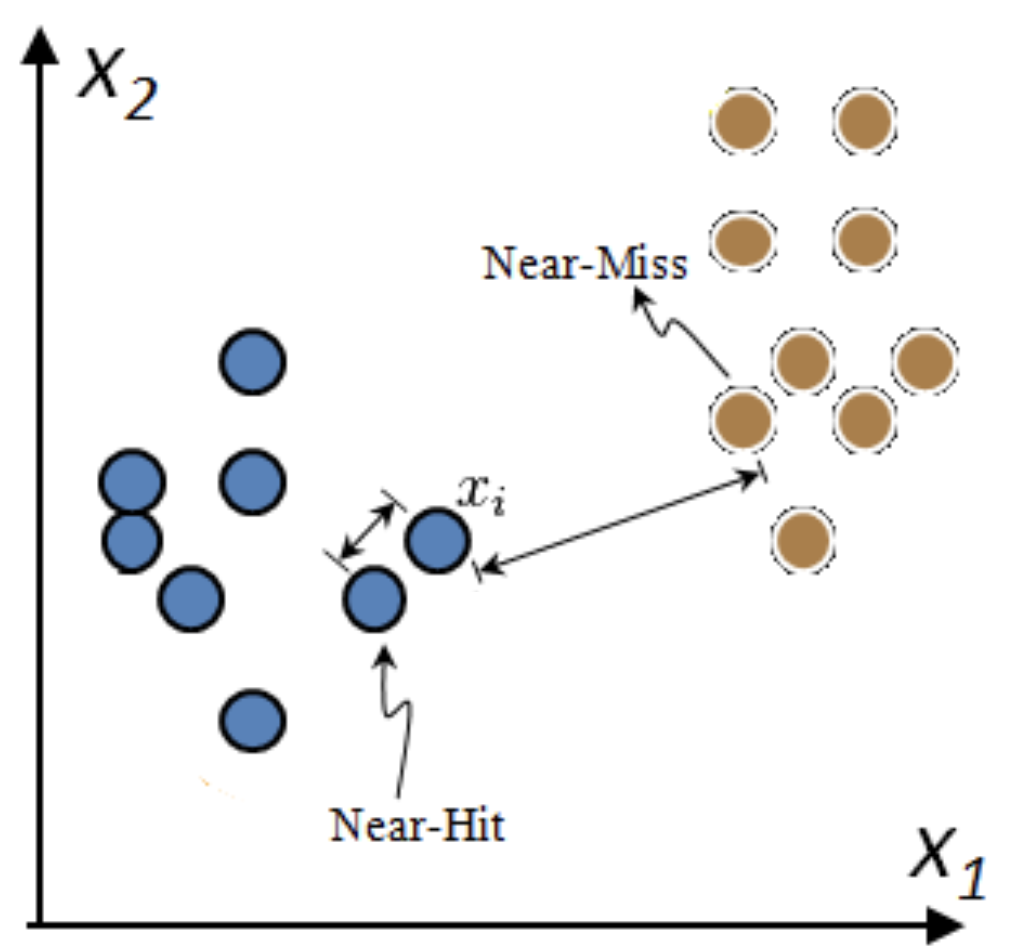
\includegraphics[width=0.75\textwidth,keepaspectratio]{images/pre-processing/relief.png}
\end{figure}
\end{frame}

\begin{frame}[allowframebreaks]{Iterative Model-based Feature Selection}
\begin{itemize}
    \item Dropping many features at once is not ideal: feature importance may change in subset
    \item Recursive Feature Elimination (RFE)
    \begin{itemize}
        \item Remove $s$ least important feature(s), recompute remaining importances, repeat
    \end{itemize}
    \item Can be rather slow
\end{itemize}

\begin{figure}
    \centering
    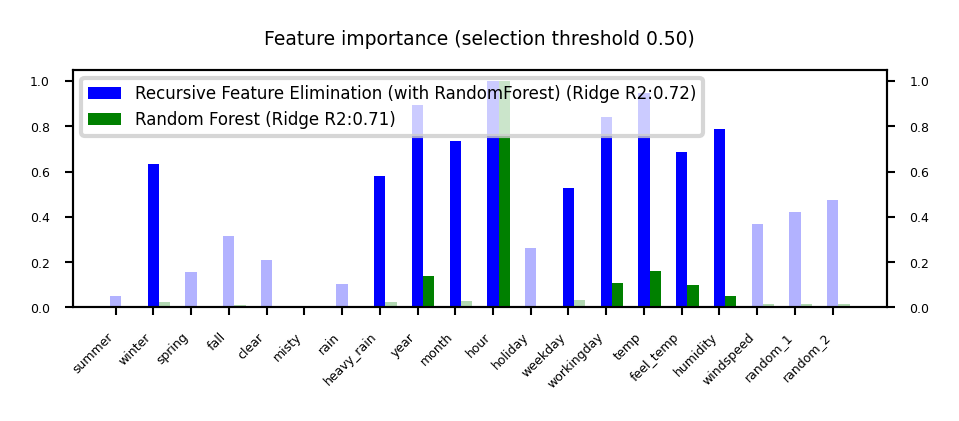
\includegraphics[width=0.9\textwidth]{images/pre-processing/iterative.png}
\end{figure}
\end{frame}


\begin{frame}[allowframebreaks]{Sequential feature selection (Wrapping)}
\begin{itemize}
    \item Evaluate your model with different sets of features, find best subset based on performance
    \item Greedy black-box search (can end up in local minima)
    \begin{itemize}
        \item Backward selection: remove least important feature, recompute importances, repeat
        \item Forward selection: set aside most important feature, recompute importances, repeat
        \item Floating: add best new feature, remove worst one, repeat (forward or backward)
    \end{itemize}
    \item Stochastic search: use random mutations in candidate subset (e.g. simulated annealing)
\end{itemize}

\begin{figure}
    \centering
    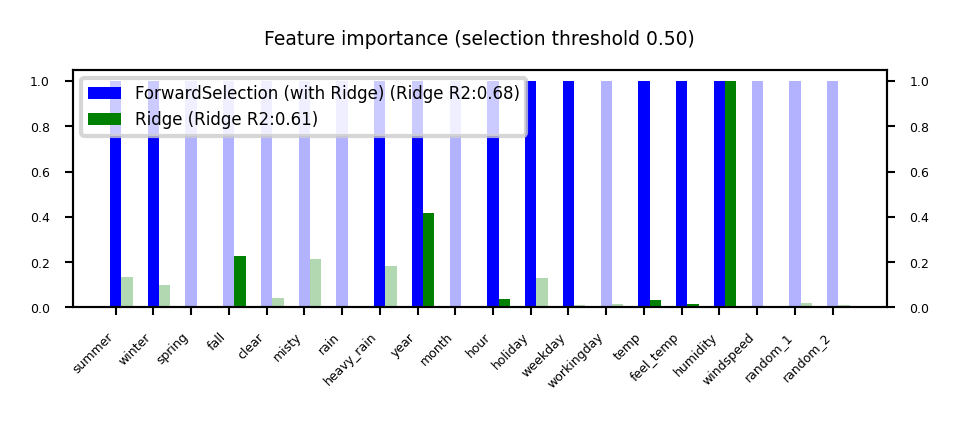
\includegraphics[width=0.9\textwidth]{images/pre-processing/sequential.png}
\end{figure}
\end{frame}

\begin{frame}[allowframebreaks]{Permutation feature importance}
\begin{itemize}
    \item Defined as the decrease in model performance when a single feature value is randomly shuffled
    \begin{itemize}
        \item This breaks the relationship between the feature and the target
    \end{itemize}
    \item Model agnostic, metric agnostic, and can be calculated many times with different permutations
    \item Can be applied to unseen data (not possible with model-based techniques)
    \item Less biased towards high-cardinality features (compared with RandomForests)
\end{itemize}

\begin{figure}
    \centering
    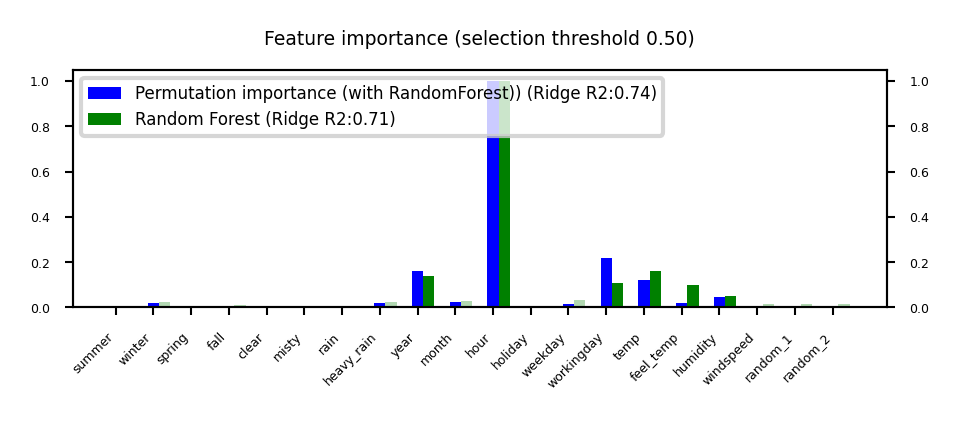
\includegraphics[width=0.9\textwidth]{images/pre-processing/permutation.png}
\end{figure}
\end{frame}

\begin{frame}[allowframebreaks]{Comparison}
\begin{itemize}
    \item Feature importances (scaled) and cross-validated \( R^2 \) score of pipeline
    \begin{itemize}
        \item Pipeline contains feature selection + Ridge
    \end{itemize}
    \item Selection threshold value ranges from 25\% to 100\% of all features
    \item Best method ultimately depends on the problem and dataset at hand
\end{itemize}

\begin{figure}
    \centering
    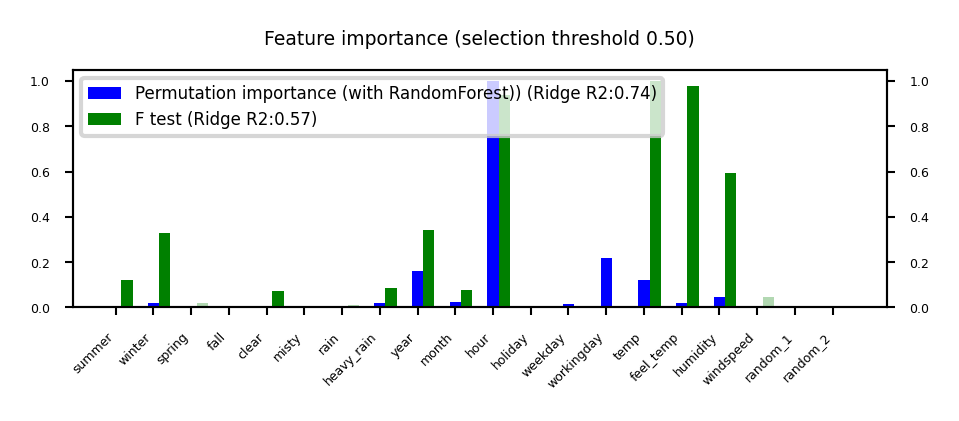
\includegraphics[width=0.9\textwidth]{images/pre-processing/comparison.png}
\end{figure}
\end{frame}





% \begin{frame}[fragile, allowframebreaks]{In practice (scikit-learn)}

% \begin{itemize}
%     \item Unsupervised: \texttt{VarianceThreshold}
% \end{itemize}

% \begin{verbatim}
% selector = VarianceThreshold(threshold=0.01)
% X_selected = selector.fit_transform(X)
% variances = selector.variances_
% \end{verbatim}

% \begin{itemize}
%     \item Univariate:
%     \begin{itemize}
%         \item For regression: \texttt{f\_regression}, \texttt{mutual\_info\_regression}
%         \item For classification: \texttt{f\_classification}, \texttt{chi2}, \texttt{mutual\_info\_classification}
%         \item Selecting: \texttt{SelectKBest}, \texttt{SelectPercentile}, \texttt{SelectFpr}, \ldots
%     \end{itemize}
% \end{itemize}

% \begin{verbatim}
% selector = SelectPercentile(score_func=f_regression, 
%                             percentile=50)
% X_selected = selector.fit_transform(X,y)
% selected_features = selector.get_support()
% f_values, p_values = f_regression(X,y)
% mi_values = mutual_info_regression(X,y,discrete_features=[])
% \end{verbatim}

% \framebreak

% \begin{itemize}
%     \item Model-based:
%     \begin{itemize}
%         \item \texttt{SelectFromModel}: requires a model and a selection threshold
%         \item \texttt{RFE}, \texttt{RFECV} (recursive feature elimination): requires model and final nr features
%     \end{itemize}
% \end{itemize}

% \begin{verbatim}
% selector = SelectFromModel(RandomForestRegressor(),
%                            threshold='mean')
% rfe_selector = RFE(RidgeCV(), n_features_to_select=20)
% X_selected = selector.fit_transform(X)
% rf_importances = RandomForest().fit(X, y).feature_importances_
% \end{verbatim}

% \begin{itemize}
%     \item Sequential feature selection (from \texttt{mlxtend}, sklearn-compatible)
% \end{itemize}

% \begin{verbatim}
% selector = SequentialFeatureSelector(RidgeCV(), k_features=20,
%                                      forward=True,
%                                      floating=True)

% X_selected = selector.fit_transform(X)
% \end{verbatim}

% \begin{itemize}
%     \item Permutation Importance (in \texttt{sklearn.inspection}), no fit-transform interface
% \end{itemize}

% \begin{verbatim}
% importances = permutation_importance(
%     RandomForestRegressor().fit(X,y),
%     X, y, n_repeats=10).importances_mean
% feature_ids = (-importances).argsort()[:n]
% \end{verbatim}

% \end{frame}
